\documentclass[conference]{IEEEtran}
\IEEEoverridecommandlockouts
% The preceding line is only needed to identify funding in the first footnote. If that is unneeded, please comment it out.
\usepackage{cite}
\usepackage{amsmath,amssymb,amsfonts}
\usepackage{algorithmic}
\usepackage{graphicx}
\usepackage{textcomp}
\usepackage{xcolor}
\usepackage{listings}
\def\BibTeX{{\rm B\kern-.05em{\sc i\kern-.025em b}\kern-.08em
    T\kern-.1667em\lower.7ex\hbox{E}\kern-.125emX}}
\begin{document}

\title{Identification of Digits from Sign Language Images
{\small Aprendizagem Automática -- Professor: Pétia Georgieva}
}

\author{\IEEEauthorblockN{José Santos, 98279}
\IEEEauthorblockA{\textit{DETI} \\
\textit{Universidade de Aveiro}}
\and
\IEEEauthorblockN{Henrique Sousa, 98324}
\IEEEauthorblockA{\textit{DETI} \\
\textit{Universidade de Aveiro}}
}

\maketitle

\begin{abstract}
    The purpose of this work is to implement and
    compare machine learning models capable of identifying digits from sign language images.
    In this paper, we tried to obtain a good result with the models using
    a dataset provided by Kaggle. Some changes are discussed,
    based on the work of others that positively affected our
    work.
\end{abstract}

\begin{IEEEkeywords}
Sign language recognition, Digit recognition, Machine learning
\end{IEEEkeywords}

\section{Introduction}
In recent years, there has been growing interest in using machine learning to develop computer vision systems capable of recognizing sign language gestures. Such systems could be used to improve communication between hearing and non-hearing individuals, as well as to facilitate the development of new technologies for the deaf and hard-of-hearing community.

In this paper, we present a novel approach to digit recognition from sign language images using machine learning. We explore several different models, including neural networks, support vector machines, and decision trees, and compare their performance on a dataset of sign language images. We also investigate the impact of some preprocessing techniques.

\section{State of the art}
Over the past few years, there have been several studies and projects focused on recognition from sign language images using machine learning techniques. Many of these approaches have utilized deep learning methods such as convolutional neural networks (CNNs), which have been shown to be effective in image recognition tasks.


\textcolor{red}{TODO: Add some references to the state of the art}
\section{Dataset Analysis}
For the development of this work, we used a dataset provided by Kaggle that contains 2062 images of sign language digits. The dataset is well balanced, with a minimum of 204 examples for a label and a maximum of 208, ensuring that every label has a similar number of examples (Figure \ref{fig:dataset-balanced}). The dataset includes data for the digits 0 to 9, resulting in 10 labels in total as we can see on the figure \ref{fig:dataset-examples}. 

\begin{figure}[h]
    \centering
    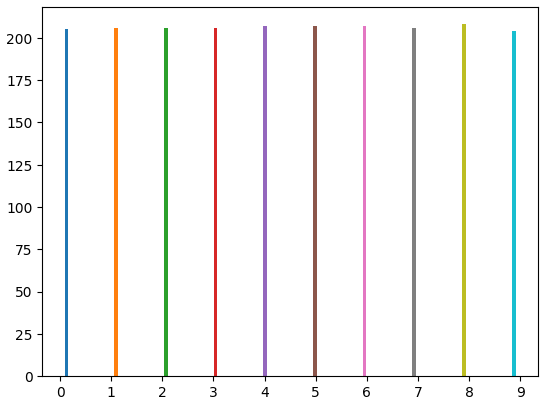
\includegraphics[width=0.4\textwidth]{assets/dataset-labels.png}
    \caption{Dataset balanced distribution}
    \label{fig:dataset-balanced}
\end{figure}


\begin{figure}[h]
    \centering
    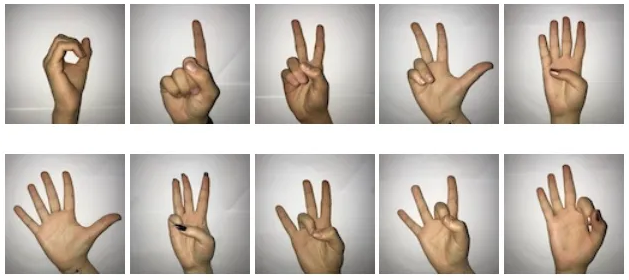
\includegraphics[width=0.4\textwidth]{assets/sign-language-digits.png}
    \caption{Dataset label examples}
    \label{fig:dataset-examples}
\end{figure}

The images are provided in a \textit{.npy} format, but we found it easier to work with the raw images to manipulate them and apply preprocessing techniques to improve the model's performance. The dataset's size and balanced distribution make it an ideal choice for training and evaluating machine learning models for digit recognition from sign language images.

\section{Dataset Preprocessing}

\subsection{Image Augmentation}
The first thing we did to the images was to augment them to create more data for model training. 
We used \textit{imgaug.augmenters} to perform the augmentation. 
The following changes were made to the images:
\begin{itemize}
    \item \textit{\textbf{Rotate}} - Rotate the image by a random angle between -20 and 20 degrees.
    \item \textit{\textbf{Gaussian noise}} - Add gaussian noise with standard deviation of 0 to 0.05*255
    \item \textit{\textbf{Gamma contrast}} - Change the contrast of the image by a random factor between 0.5 and 1.5.
\end{itemize}
For every image in the dataset, we created 5 new images with the above changes. Due to the small size of the dataset, we decided to perform the augmentation offline, before splitting the dataset into training and test data.

\subsection{Image Preprocessing}
We also resized the images to 50x50 pixels (down from the original size of 64x64), as we found that this size was sufficient for the models to achieve good results. Then, we converted the images to grayscale and flattened them, as we found that this improved the performance of the models.

Finally, we split the dataset into training and test data. We used an 80/20 split, with 80\% of the data being used for training and 20\% for testing.
Resulting in 9897 total images for the training data and 2475 for the test data.

\begin{figure}[!h]
    \centering
    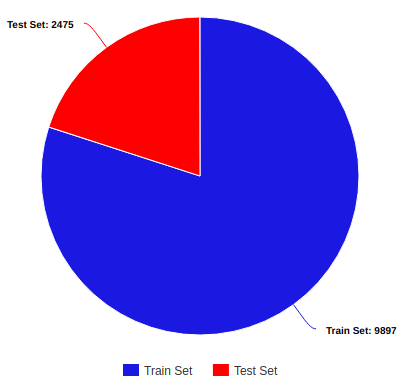
\includegraphics[width=0.3\textwidth]{assets/meta-chart.png}
    \caption{Dataset Distribution}
    \label{fig:dataset-dist}
\end{figure}
\section{Models}
In order to find the best training model, we tested several different models, including neural networks, support vector machines, and decision trees. We also tested different preprocessing techniques to see if they had any impact on the model's performance as discussed before.
The two evaluation metrics used to measure the performance of the models are Accuracy and F1 Score. Accuracy is the proportion of correct predictions over the total number of predictions, while F1 Score considers both precision and recall of the model's predictions.

First, we tried a lot of models with their default parameters to understand which ones had value
and were worth to be improved. These were the first results: 

\begin{table}[!h]
    \centering
    \label{tab:models-default-parameters}
    \begin{tabular}{|l|c|c|}
    \hline
    \textbf{Model}                                                                                  & \textbf{Accuracy} & \textbf{F1 Score} \\ \hline
    Logistic Regression                                                                             & 0.750             & 0.749             \\ \hline
    Decision Tree Classifier                                                                        & 0.631             & 0.632             \\ \hline
    Random Forest Classifier                                                                        & 0.876             & 0.876             \\ \hline
    Naive Bayes                                                                                     & 0.502             & 0.506             \\ \hline
    Support Vector Machines                                                                         & 0.888             & 0.888             \\ \hline
    \begin{tabular}[c]{@{}l@{}}Neural Networks\\ (Multilayer Perceptron \\ Classifier)\end{tabular} & 0.092             & 0.015             \\ \hline
    \end{tabular}
    \caption{Models' performance with default parameters}
\end{table}

Among all the models, Support Vector Machines has the highest accuracy and F1 Score, both of which are 0.888. Random Forest Classifier also shows a good performance with accuracy and F1 Score of 0.876. Logistic Regression comes in third place with accuracy and F1 Score of 0.750 and 0.749, respectively.
The other models have lower performance, so for the next step, we will skip the Decision Tree Classifier and Naive Bayes. 
We will still try to find ideal parameters for the MLP Classifier because the model ended up predicting the same label for each example. This is probably because the model was not trained properly, so we will give it a chance and try to improve it.

\subsection{Hyperparameter Tuning \& Cross-Validation}
Hyperparameter tuning is the process of finding the best values for the parameters that result in the best performance of the model on the given dataset.
The purpose of cross-validation is to estimate how well a machine learning model will generalize to new data. By evaluating the model on multiple subsets of the data, it is less likely that the model's performance is biased towards a particular subset of the data. Cross-validation is commonly used in machine learning to evaluate the performance of different models or to compare the performance of different hyperparameters.
To implement these methods and get the best model performance, we created a function that given a model, the parameters to test and the dataset, it will try the different combinations of parameters and return the best model and its performance. The function also performs cross-validation on the training data to evaluate the model's performance. The following code shows the function's implementation:

\begin{lstlisting}[language=Python]
def hyperparameters(model, params, X, y):
    model = GridSearchCV(model, params, 
    scoring="accuracy")
    model.fit(X, y)
    print("Best Parameters:")
    print(model.bestparams)
\end{lstlisting}

These function is going to be applied in the models with different parameters to find the best model for each one.

\subsection{Support Vector Machines}
Support Vector Machines (SVM) proved to be the best-performing model for the classification task, with an initial accuracy and F1 Score of 88.8\% using default parameters. In an effort to improve the performance of the SVM model, we experimented with different values for the C, kernel, degree, and gamma parameters, as shown in Table~\ref{tab:svm_parameters}.

\begin{table}[!h]
    \centering
    \label{tab:svm_parameters}
    \begin{tabular}{|c|l|c|}
    \hline
    \textbf{Parameter} & \multicolumn{1}{c|}{\textbf{Values}}     & \multicolumn{1}{l|}{\textbf{Best Value}} \\ \hline
    C                  & {[}0.001, 0.01, 0.1, 1, 10, 100, 1000{]} & 100                                      \\ \hline
    kernel             & {[}linear, poly, rbf, sigmoid{]}         & rbf                                      \\ \hline
    degree             & {[}2, 3, 4, 5{]}                         & 2                                        \\ \hline
    gamma              & {[}scale, auto{]}                        & scale                                    \\ \hline
    \end{tabular}
    \caption{SVM Parameters}
\end{table}

After running several iterations, we were able to identify the optimal parameter values, which resulted in a significant improvement in performance. The best-performing parameters were: 

\begin{itemize}
    \item \textbf{C} = 100
    \item \textbf{kernel} = rbf
    \item \textbf{degree} = 2
    \item \textbf{gamma} = scale
\end{itemize}
The SVM model with these parameters achieved an accuracy and F1 Score of 95\%, which represents a significant improvement over the default parameters.
We can better visualize the performance of the SVM model by looking at the confusion matrix, as shown in Figure~\ref{fig:svm_confusion_matrix}.

\begin{figure}[!h]
    \centering
    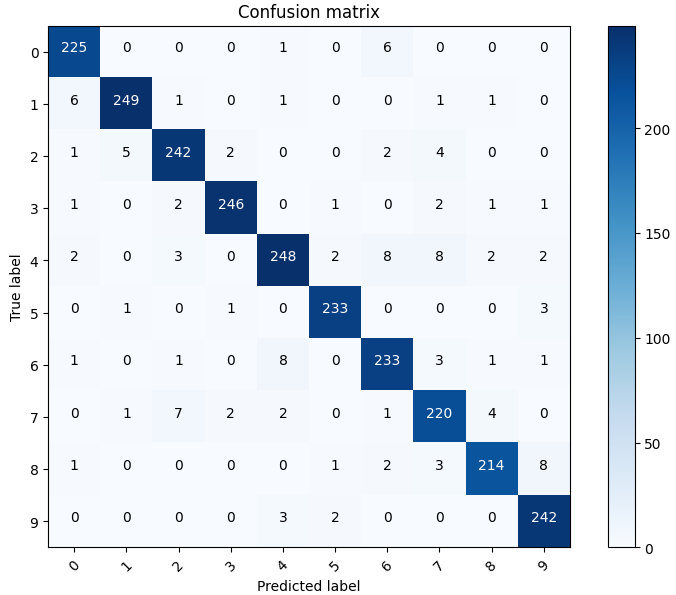
\includegraphics[width=0.5\textwidth]{assets/svm-confusion-matrix.png}
    \caption{SVM Confusion Matrix}
    \label{fig:svm_confusion_matrix}
\end{figure}

As we can see in the confusion matrix, the SVM model can correctly classify most of the images. 
Some classes are misclassified. This is probably because the images of these classes are very similar to each other, so it is not surprising that the model has a hard time classifying them correctly.
\begin{table}[!h]
    \centering
    \begin{tabular}{|c|c|c|c|r|}
        \hline
        \textbf{Label} & \textbf{Precision} & \textbf{Recall} &  \textbf{F1 Score} \\ \hline
        0              & 0.95               & 0.97            & 0.96               \\ \hline
        1              & 0.97               & 0.96            & 0.97               \\ \hline
        2              & 0.95               & 0.95            & 0.95               \\ \hline
        3              & 0.98               & 0.97            & 0.97               \\ \hline
        4              & 0.94               & 0.90            & 0.92               \\ \hline
        5              & 0.97               & 0.98            & 0.98               \\ \hline
        6              & 0.92               & 0.94            & 0.93               \\ \hline
        7              & 0.91               & 0.93            & 0.92               \\ \hline
        8              & 0.96               & 0.93            & 0.95               \\ \hline
        9              & 0.94               & 0.98            & 0.96               \\ \hline
    \end{tabular}
    \label{tab:svm_classification_report}
    \caption{SVM Classification Report}
\end{table}
Looking at the precision scores, which measure the proportion of true positives among all samples predicted as positive, we can see that the model performed well for most classes, with scores ranging from 0.91 to 0.98. This indicates that when the model predicted a certain class, it was usually correct.

The recall scores, which measure the proportion of true positives among all actual positive samples, are also high for most classes, ranging from 0.90 to 0.98. This suggests that the model was able to identify most instances of each class correctly.

In addition to high precision and recall scores, the F1-score, which balances these two metrics, also indicates strong performance for most classes, with scores ranging from 0.92 to 0.98. This suggests that the model achieved a good trade-off between precision and recall, and is able to correctly classify samples while minimizing false positives and false negatives.
Overall, these results suggest that the classification model was effective at distinguishing between the different classes in the dataset, with high levels of precision, recall, and F1-score for most classes.

\subsection{Random Forest Classifier}
The Random Forest Classification model was the second best model with the default parameters and was very close to the SVM model, initially. 
The accuracy and F1 Score were 88.8\%. 
In an effort to improve the accuracy of this model. 
We experimented with different values for the model parameters, as shown in Table~\ref{tab:rf_parameters}.
\begin{table}[!h]
    \centering
    \label{tab:rf_parameters}
    \begin{tabular}{|c|l|c|}
    \hline
    \textbf{Parameter} & \multicolumn{1}{c|}{\textbf{Values}}     & \multicolumn{1}{l|}{\textbf{Best Value}} \\ \hline
    n\_estimators       & {[}50, 100, 200, 500{]}                  & 500                                      \\ \hline
    criterion          & {[}gini, entropy{]}                      & entropy                                  \\ \hline
    max\_depth          & {[}None, 5, 10, 20{]}                    & None                                     \\ \hline
    min\_samples\_split  & {[}2, 5, 10{]}                           & 2                                   \\ \hline
    min\_samples\_leaf   & {[}1, 2, 4{]}                            & 1                                 \\ \hline
    max\_features       & {[}auto, sqrt, log2{]}                   & auto                                    \\ \hline
    \end{tabular}
    \caption{Random Forest Classifier Parameters}
\end{table}

As we see in the table above, the best parameters for the Random Forest Classifier were:

\begin{itemize}
    \item \textbf{n\_estimators} = 500
    \item \textbf{criterion} = entropy
    \item \textbf{max\_depth} = None
    \item \textbf{min\_samples\_split} = 2
    \item \textbf{min\_samples\_leaf} = 1
    \item \textbf{max\_features} = auto
\end{itemize}

The Random Forest Classifier model with these parameters achieved an accuracy and F1 Score of 89.1\%. The selection of ideal parameters only barely improved the model over the default parameters.
By looking at the confusion matrix in figure \ref{fig:rf_confusion_matrix}, we can confirm that the model performed decently in classifying the images of sign language digits.
\begin{figure}[!h]
    \centering
    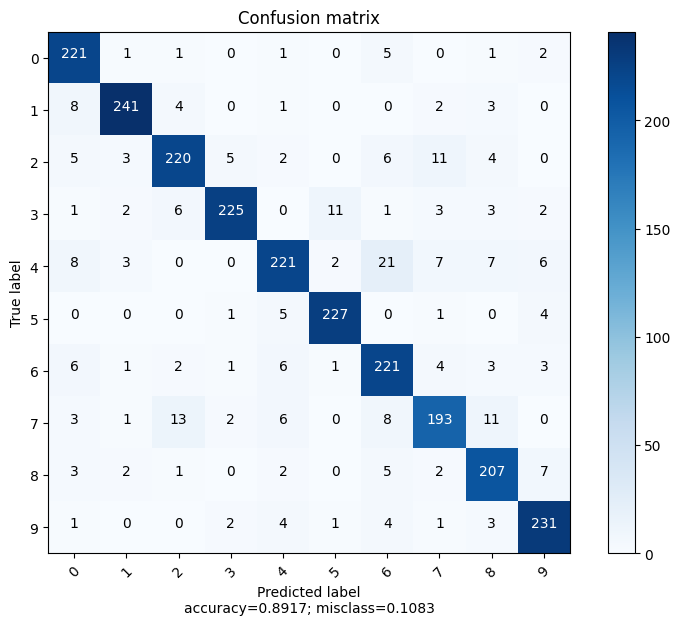
\includegraphics[width=0.5\textwidth]{assets/rfc-confusion-matrix.png}
    \caption{Random Forest Confusion Matrix}
    \label{fig:rf_confusion_matrix}
\end{figure}

In table \ref{tab:rfc_classification_report} we can check the precision, recall and f1 score for each label in the dataset.

\begin{table}[!h]
    \centering
    \begin{tabular}{|c|c|c|c|r|}
        \hline
        \textbf{Label} & \textbf{Precision} & \textbf{Recall} & \textbf{F1 Score} \\ \hline
        0              & 0.86               & 0.95            & 0.91              \\ \hline
        1              & 0.95               & 0.93            & 0.94              \\ \hline
        2              & 0.89               & 0.86            & 0.87              \\ \hline
        3              & 0.95               & 0.89            & 0.92              \\ \hline
        4              & 0.89               & 0.80            & 0.85              \\ \hline
        5              & 0.94               & 0.95            & 0.95              \\ \hline
        6              & 0.82               & 0.89            & 0.85              \\ \hline
        7              & 0.86               & 0.81            & 0.84              \\ \hline
        8              & 0.86               & 0.90            & 0.88              \\ \hline
        9              & 0.91               & 0.94            & 0.92              \\ \hline
    \end{tabular}
    \label{tab:rfc_classification_report}
    \caption{Random Forest Classification Report}
\end{table}

\textcolor{red}{ADD COST LOSS OVER ITERATIONS FOR EVERY MODEL}

\subsection{Multilayer Perceptron}
This Neural Network approach was the model that delivered the worst results with the default parameters with a very bad accuracy and f1 socre of 0.092 and 0.015, respectively.
The model got these values because it was not able to predict the labels correctly and kept predicting every image with the same label. This could be indicating that our model was not able to converge in order to understand how to diferentiate every label,
so we didn't discard it in the initial phase and tried to get better results with it.
This model is resource intensive so we were not able to test every possible combination of the parameters seen on table \ref{tab:mlp_parameters} below.

\begin{table}[!h]
    \centering
    \label{tab:mlp_parameters}
    \begin{tabular}{|c|l|c|}
    \hline
    \textbf{Parameter} & \multicolumn{1}{c|}{\textbf{Values}}     & \multicolumn{1}{l|}{\textbf{Best Value}} \\ \hline
    solver       & {[}adam, lbfgs{]}                  & lbfgs                                      \\ \hline
    max\_iter          & {[}250, 500, 1000{]}                      & 1000                                  \\ \hline
    hidden\_layer\_sizes         & {[}(128,), (256,), (512,), (128, 128), (256, 256), (512, 512), (128, 256, 512), (128, 512, 256), (512, 256, 128){]}                    & (256, 512, 128)                                     \\ \hline
    activation  & {[}relu, tanh{]}                           & relu                                   \\ \hline
    alpha   & {[}0.0001, 0.001, 0.01{]}                            & 0.0001                               \\ \hline
    learning\_rate       & {[}constant, invscaling, adaptive{]}                   & adaptive                                    \\ \hline
    learning\_rate\_init    & {[}0.001, 0.01, 0.1{]}                   & 0.001                                    \\ \hline
    \end{tabular}
    \caption{Multilayer Perceptron Parameters}
\end{table}

So we tried manually without using the hyperparameters function we developed some combinations with the parameters seen below.
The best results we got were with the parameters seen below:
\begin{itemize}
    \item \textbf{solver} = lbfgs
    \item \textbf{max\_iter} = 1000
    \item \textbf{hidden\_layer\_sizes} = (256, 512, 128)
    \item \textbf{activation} = relu
    \item \textbf{alpha} = 0.0001
    \item \textbf{learning\_rate} = adaptive
    \item \textbf{learning\_rate\_init} = 0.001
\end{itemize}

These parameters produced better results than the ones seen above, generating the confusion matrix in figure \ref{fig:mlp_confusion_matrix}.

\begin{figure}[!h]
    \centering
    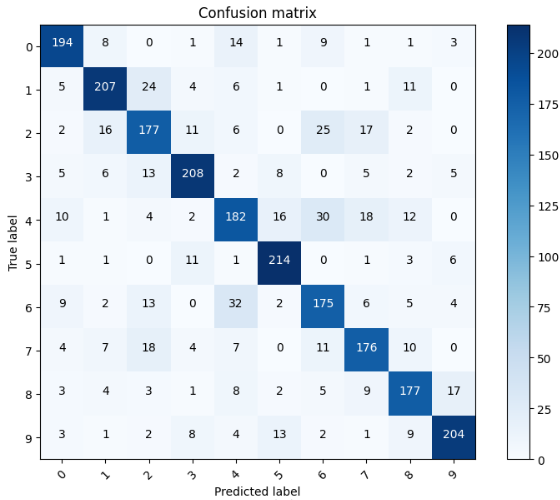
\includegraphics[width=0.5\textwidth]{assets/mlp-confusion-matrix.png}
    \caption{MLP Confusion Matrix}
    \label{fig:mlp_confusion_matrix}
\end{figure}

As we can see, now the model is able to diferentiate the different labels, but still missclassified a lot of examples which resulted in a accuracy and f1 score of 77,3\%.
Although, this was the best improvement comparing with the model with the default parameters it is still far from being the best performing model for these problem.
The precision, recall and f1 score for each label can be observed below in table \ref{tab:mlp_classification_report}.

\begin{table}[!h]
    \centering
    \begin{tabular}{|c|c|c|c|r|}
        \hline
        \textbf{Label} & \textbf{Precision} & \textbf{Recall} & \textbf{F1 Score} \\ \hline
        0              & 0.82               & 0.84            & 0.83              \\ \hline
        1              & 0.82               & 0.80            & 0.81              \\ \hline
        2              & 0.70               & 0.69            & 0.69              \\ \hline
        3              & 0.83               & 0.82            & 0.83              \\ \hline
        4              & 0.69               & 0.66            & 0.68              \\ \hline
        5              & 0.83               & 0.90            & 0.86              \\ \hline
        6              & 0.68               & 0.71            & 0.69              \\ \hline
        7              & 0.75               & 0.74            & 0.75              \\ \hline
        8              & 0.76               & 0.77            & 0.77              \\ \hline
        9              & 0.85               & 0.83            & 0.84              \\ \hline
    \end{tabular}
    \label{tab:mlp_classification_report}
    \caption{Multilayer Perceptron Report}
\end{table}



\subsection{Logistic Regression}

\section{Model comparison}

\subsection{Image Augmentation Result}
\section{Conclusion}

\section{References}

\begin{thebibliography}{00}
    \bibitem{b1} Akanksha Telagamsetty, Sign Language Digits Classification https://medium.com/analytics-vidhya/sign-language-classification-64fe8ad0fc2c
\end{thebibliography}

\end{document}
